	\documentclass[aspectratio=169]{beamer}
\usepackage[utf8]{inputenc}
\usepackage[T1]{fontenc}
\usepackage[brazil]{babel}
\usepackage{graphics,amssymb,amsfonts,amsmath}
\usepackage{tikz}
\usepackage{enumerate,hyperref}
\usepackage{palatino}
\usepackage{ragged2e}
\usepackage{minted}
\usepackage{booktabs}

\usetheme{AnnArbor}
\usecolortheme{orchid}
\usefonttheme[onlymath]{serif}

\AtBeginSection[]{
  \begin{frame}
  \vfill
  \centering
  \begin{beamercolorbox}[sep=8pt,center,shadow=true,rounded=true]{title}
    \usebeamerfont{title}\insertsectionhead\par%
  \end{beamercolorbox}
  \vfill
  \end{frame}
}

\newminted{java}{bgcolor=cyan!10}

\title[\sc{Introdução}]{Introdução}
\author[Roland Teodorowitsch]{Roland Teodorowitsch}
\institute[FPROG - EP - PUCRS]{Fundamentos de Programação - Escola Politécnica - PUCRS}
\date{16 de maio de 2023}

\begin{document}
\justifying

%-------------------------------------------------------
\begin{frame}
	\titlepage
\end{frame}

%-------------------------------------------------------
\begin{frame}
\vspace{5cm}
\begin{flushright}
\emph{``Computers are good at\\
following instructions, but not at\\
reading your mind.''}\\
(Donald Knuth)
\end{flushright}
\end{frame}

%=======================================================
\section{Sumário}

%-------------------------------------------------------
\begin{frame}\frametitle{Sumário}
\begin{itemize}
	\item Programas de Computador
	\item A anatomia de um computador
	\item A linguagem de programação Java
	\item Familiarizando-se com o ambiente de programação
	\item Analisando seu primeiro programa
	\item Exercícios
	\item Erros
	\item Solução de problemas: projeto de algoritmos
	\item Referências
\end{itemize}
\end{frame}


%=======================================================
\section{Programas de Computador}

%-------------------------------------------------------
\begin{frame}\frametitle{Programas de computador}
\begin{itemize}
	\item \textbf{computadores}
	\begin{itemize}
		\item são máquinas usadas para automatizar a execução de tarefas
		\item computadores podem executar instruções básicas de forma bastante simples
		\item são máquinas de flexíveis e de propósito geral que podem ser usadas para diferentes atividades
		\item são máquinas que armazenam dados (números, palavras, imagens), interagem com dispositivos (monitor, sistema de som, impressora) e executam \textbf{programas}
	\end{itemize}
	\item \textbf{programa} (de computador)
	\begin{itemize}
		\item permite que um computador desempenhe funções diferentes
		\item é uma sequência de instruções/passos que diz ao computador como realizar determinada tarefa
	\end{itemize}
\end{itemize}
\end{frame}

%-------------------------------------------------------
\begin{frame}\frametitle{Programas de computador}
\begin{itemize}
	\item o computador e os dispositivos periféricos são coletivamente chamados de \textbf{hardware}
	\item o programas que o computador executa são chamados de \textbf{software}
	\item \textbf{programação} corresponde à ação de projetar e implementar programas de computador
	\item aplicações complexas são formadas por um grande número de instruções simples engenhosamente combinadas - e para implementar tais aplicações um programador precisa trilhar um caminho que inicia com o entendimento de uma série de construções mais simples (o que é o objetivo desta disciplina)
\end{itemize}
\end{frame}

%=======================================================
\section{A anatomia de um computador}

%-------------------------------------------------------
\begin{frame}\frametitle{A anatomia de um computador}
\begin{itemize}
	\item conhecer os blocos básicos que compõe um computador pode ajudar no processo de programação
	\item o \textbf{processador} ou \textbf{UCP} (Unidade Central de Processamento ou \emph{CPU}) é o coração/cérebro do computador
	\begin{itemize}
		\item é formado por um número bastante grande de elementos estruturais chamados \textbf{transistores}
		\item localiza e executa as instruções dos programas
		\item é capaz de realizar operações aritméticas, buscar dados na memória externa e salvar dados processados em unidades de armazenamento
	\end{itemize}
\end{itemize}
\begin{figure}[h]
	\centering
	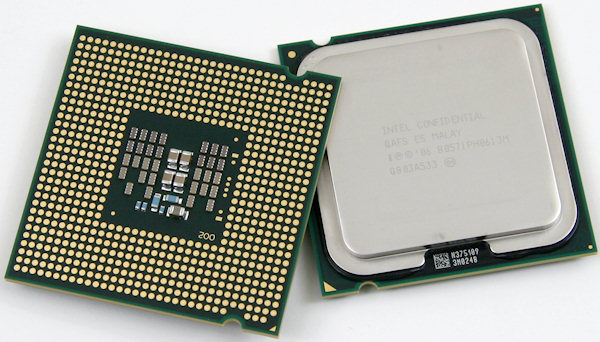
\includegraphics[height=0.25\paperheight]{pucrs-ep-fprog-unidade_01-introducao-laminas-ucp.png}
\end{figure}
\end{frame}

%-------------------------------------------------------
\begin{frame}\frametitle{A anatomia de um computador}
\begin{itemize}
	\item há 2 tipos de armazenamento
	\begin{itemize}
		\item primário: circuitos de memória que mantêm a informação enquanto estão energizados (ou seja, são voláteis)
		\item secundário: dispositivos como discos rígidos, que são mais lentos, porém são mais baratos, de maior capacidade e mantêm a informação de forma não volátil
	\end{itemize}
\end{itemize}
\begin{figure}[h]
	\centering
	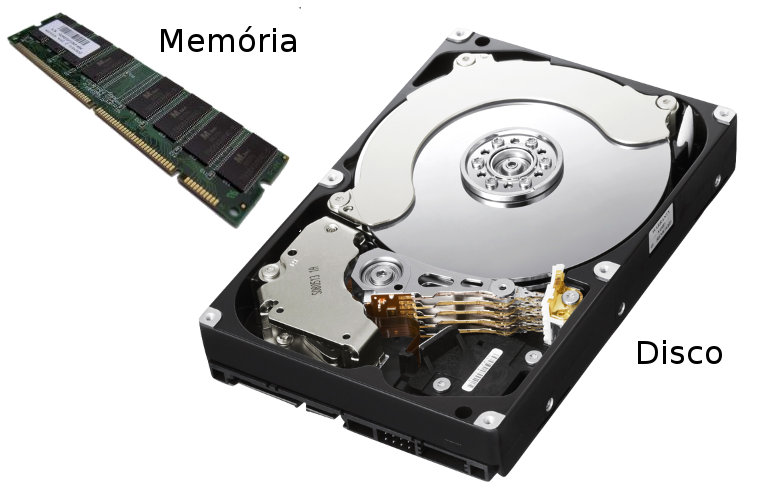
\includegraphics[height=0.45\paperheight]{pucrs-ep-fprog-unidade_01-introducao-laminas-armazenamento.jpg}
\end{figure}
\end{frame}

%-------------------------------------------------------
\begin{frame}\frametitle{A anatomia de um computador}
\begin{itemize}
	\item o computador armazena tanto dados quanto programas
	\item eles são armazenados em dispositivos de armazenamento secundário e carregados para a memória quando forem executados
	\item um programa altera os dados na memória e salva os dados modificados no armazenamento secundário
	\item para interagir com usuários humanos, um computador necessita de \textbf{periféricos} ou \textbf{dispositivos}
	\item o computador envia dados para dispositivos de saída (\emph{output}): monitor, auto-falantes, impressoras
	\item e obtém informação de dispositivos de entrada (\emph{input}): teclado, mouse
	\item computadores podem ser conectados entre si, formando uma \textbf{rede de computadores} que permite a troca de dados entre computadores
\end{itemize}
\end{frame}

%=======================================================
\section{A linguagem de programação Java}

%-------------------------------------------------------
\begin{frame}\frametitle{A linguagem de programação Java}
\begin{itemize}
	\item em vez de escrever um programa instrução por instrução, programadores usam \textbf{linguagens de alto nível}
	\item em uma linguagem de alto nível é possível usar ações que são traduzidas por um \textbf{compilador} para as instruções que o computador entende
	\item há também linguagens interpretadas, onde um \textbf{interpretador} lê as ações e as executa sem convertê-las para instruções do processador
	\item muitas linguagens têm sido desenvolvidas para as mais diferentes finalidades
\end{itemize}
\end{frame}

%-------------------------------------------------------
\begin{frame}\frametitle{Linguagens de alto nível, de montagem, de máquina}
\begin{figure}[h]
	\centering
	\includegraphics[height=0.65\paperheight]{pucrs-ep-fprog-unidade_01-introducao-laminas-computer_languages.png}\\
	\tiny{https://www.cs.mtsu.edu/~xyang/images/computer-languages.png}
\end{figure}
\end{frame}
	
%-------------------------------------------------------
\begin{frame}\frametitle{A linguagem de programação Java}
\begin{figure}[h]
	\centering
	
\includegraphics[height=0.2\paperheight]{pucrs-ep-fprog-unidade_01-introducao-laminas-java.jpg}
\end{figure}
\begin{itemize}
	\item em 1991, um grupo liderado por James Gosling e Patrick Naughton na Sun Microsystems projetou uma linguagem (codinome \emph{``Green''}) para ser usada em dispositivos de consumo, mas acabou sendo usada a partir de 1994 para escrever \textbf{applets} (código Java que pode ser obtido da Internet e executado localmente por um navegador)
	\item a linguagem passou a ser chamada de Java e cresceu muito desde então
\end{itemize}
\end{frame}

%-------------------------------------------------------
\begin{frame}\frametitle{A linguagem de programação Java}
\begin{itemize}
	\item Java possui uma \textbf{biblioteca} rica que permite escrever programas portáveis
	\item edições variando de \emph{``micro''} a \emph{``enterprise''} permitem escrever programas em Java para todas as necessidades (\emph{smart cards}, telefones celulares, servidores)
	\item como foi projetada para a Internet, possui um foco forte na segurança e na portabilidade
	\item Java consegue ser portável pois não converte o código-fonte diretamente para instruções do processador, mas para \textbf{bytecodes} que são interpretados por uma \textbf{máquina virtual} Java
\end{itemize}
\end{frame}

%=======================================================
\section{Familiarizando-se com o ambiente de programação}

%-------------------------------------------------------
\begin{frame}\frametitle{Familiarizando-se com o ambiente de programação}
\begin{itemize}
	\item há muitas maneiras de se programar em Java:
	\begin{itemize}
		\item usar um \textbf{editor} simples (\texttt{notepad}, \texttt{vi}, \texttt{gedit}), chamando o compilador (\texttt{javac}) e a seguir executando o programa compilado (\texttt{java})
		\item usar um \textbf{IDE} (\emph{Integrated Development Environment}), tal como BlueJ, Eclipse, NetBeans, etc.
	\end{itemize}
	\item vamos começar com o modo mais ``rústico''...
\end{itemize}
\end{frame}

%-------------------------------------------------------
\begin{frame}[fragile]\frametitle{Usando a linha de comando}
\begin{itemize}
	\item use um editor qualquer para digitar o seguinte código:
\begin{javacode}
public class MeuPrimeiroPrograma {
  public static void main (String[] args) {
    System.out.println("Este e' o meu primeiro programa...");
  }
}
\end{javacode}
	\item ATENÇÃO: mantenha as letras maiúsculas e minúsculas literalmente conforme o exemplo!
\end{itemize}
\end{frame}

%-------------------------------------------------------
\begin{frame}\frametitle{Usando a linha de comando}
\begin{itemize}
	\item abra um interpretador de comandos e vá para o diretório onde você salvou o arquivo
	\item salve-o com o nome \texttt{MeuPrimeiroPrograma.java}
	\item compile-o com \texttt{javac MeuPrimeiroPrograma.java}
	\item rode-o com \texttt{java MeuPrimeiroPrograma}
	\item certifique-se que o ambiente java esteja no PATH (caso não esteja, use o caminho completo até os arquivos \texttt{javac} e \texttt{java})
	\item NÃO funcionou? NÃO se desespere o professor vai mostrar como fazer.
\end{itemize}
\end{frame}

%-------------------------------------------------------
\begin{frame}\frametitle{Usando o BlueJ}
\begin{itemize}
	\item agora com o...
	\begin{figure}[h]
		\centering
		
\includegraphics[height=0.5\paperheight]{pucrs-ep-fprog-unidade_01-introducao-laminas-bluej_logo.jpg}
	\end{figure}
\end{itemize}
\end{frame}

%-------------------------------------------------------
\begin{frame}\frametitle{Usando o BlueJ}
\begin{itemize}
	\item abra o BlueJ:
	\begin{figure}[h]
		\centering
		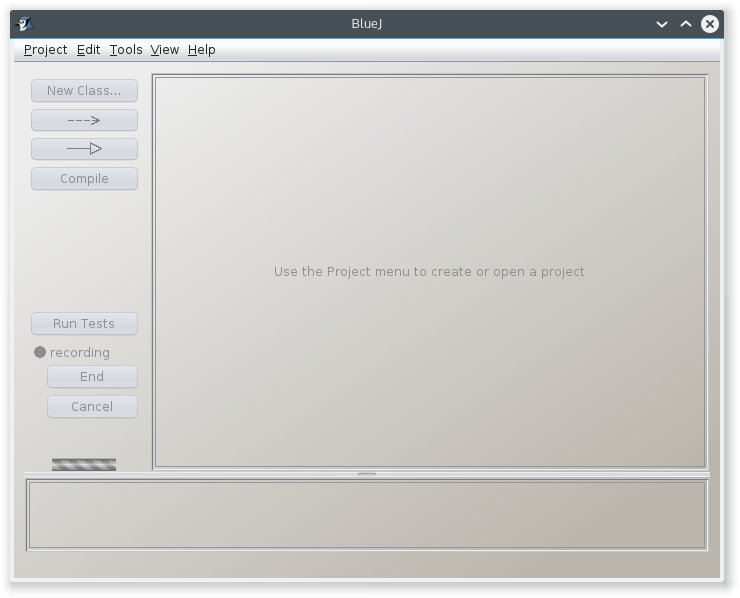
\includegraphics[height=0.65\paperheight]{pucrs-ep-fprog-unidade_01-introducao-laminas-bluej.jpg}
	\end{figure}
\end{itemize}
\end{frame}

%-------------------------------------------------------
\begin{frame}\frametitle{Usando o BlueJ}
\begin{itemize}
	\item selecione \texttt{\underline{P}roject} e \texttt{\underline{N}ew Project}
	\item crie um diretório novo para o seu projeto (por exemplo: \texttt{MeuSegundoPrograma}) e selecione o botão \texttt{Create}
	\item use o botão \texttt{New Class} para criar uma nova classe (por exemplo: \texttt{MeuSegundoPrograma})
	\item com o botão direito do mouse, clique duas vezes a caixa criada
\end{itemize}
\end{frame}

%-------------------------------------------------------
\begin{frame}[fragile]\frametitle{Usando o BlueJ}
\begin{itemize}
	\item substitua o código por:
\begin{javacode}
/*
 * Este e' um comentario de varias linhas
 * (podem ocorrer problemas com acentos...)
 */
public class MeuSegundoPrograma {
  public static void main (String[] args) {
    // Este e' um comentario de uma linha
    System.out.println("A cada dia aprendo coisas novas...");
  }
}
\end{javacode}
	\item pressione o botão \texttt{Compile} (preste atenção para verificar se não houve erros de digitação)
\end{itemize}
\end{frame}

%-------------------------------------------------------
\begin{frame}\frametitle{Usando o BlueJ}
\begin{itemize}
	\item pressione o botão \texttt{Close} da janela de edição da ``classe'' e volte para a janela do projeto
	\item abra o menu de opções clicando com o botão direito do \emph{mouse} sobre a caixa da classe que foi criada, selecione a segunda opção: ``\texttt{void main(String[] args)}'' e, a seguir, pressione o botão \texttt{Ok}
\end{itemize}
\end{frame}

%-------------------------------------------------------
\begin{frame}\frametitle{Considerações}
\begin{itemize}
	\item \texttt{javac} converte o código-fonte em linguagem de alto nível em um arquivo \texttt{.class} (que contém instruções para a máquina virtual Java)
	\item \texttt{java} executa o arquivo \texttt{.class} na máquina virtual Java
	\item em uma IDE, tudo isto é feito de forma transparente
\end{itemize}
\begin{figure}[h]
\centering
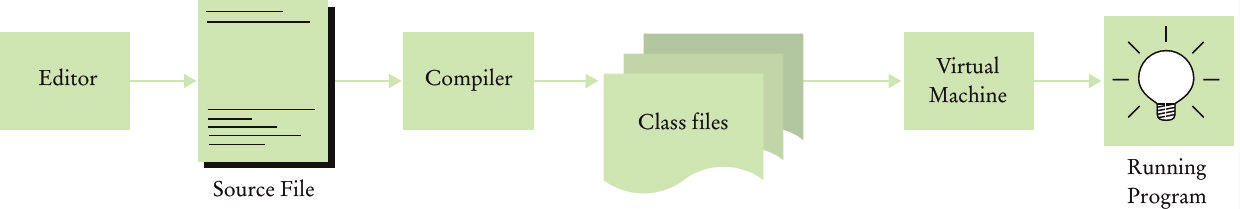
\includegraphics[height=0.25\paperheight]{pucrs-ep-fprog-unidade_01-introducao-laminas-compilacao.jpg}\\
(HORSTMANN, 2013, p. 9)
\end{figure}
\end{frame}

%-------------------------------------------------------
\begin{frame}\frametitle{Organize-se}
\begin{itemize}
	\item você pode aproveitar o \emph{template} que o BlueJ gera ao se criar uma classe e usá-lo como padrão para seus futuros programas
	\item programas (em código-fonte ou já convertidos em instruções) são armazenados em arquivos e para manter estes arquivos bem organizados é importante criar uma hierarquia de diretórios (ou pastas)
	\item por exemplo, dentro do seu diretório de documentos crie um subdiretório para a universidade
	\item dentro do subdiretório da universidade, crie um subdiretório para cada disciplina
	\item dentro do subdiretório da disciplina, crie subdiretórios para apostilas, exercícios, trabalhos, etc.
	\item dentro do subdiretório de exercícios, crie um subdiretório para cada exercício
\end{itemize}
\end{frame}

%-------------------------------------------------------
\begin{frame}\frametitle{Faça cópias de segurança (\emph{backups})}
\begin{itemize}
	\item você vai perder muito tempo escrevendo programas, então é bom certificar-se de nada de errado vai acontecer com eles
	\item faça cópias de segurança (em \emph{pen drives}, no \emph{smartphone}, na Internet ou onde achar melhor)
	\item se for um projeto maior, mantenha um histórico de {\emph backups} (por exemplo, com \emph{backups} diários não sobrepostos) - pode-se também criar um mecanismo de rotação
	\item faça \emph{backups} com frequência
	\item certifique-se de que o \emph{backups} funcionou
	\item tome cuidado para que ninguém roube os dados do seu \emph{backup}
	\item se ocorrer algum problema com seus arquivos, relaxe e recupere-o do \emph{backup}
\end{itemize}
\end{frame}

%-------------------------------------------------------
\begin{frame}\frametitle{Não se assuste...}
Java é uma linguagem poderosa e que, em um primeiro momento, pode parecer complicada.
Por isso os conceitos, comandos e recursos da linguagem serão apresentados, explicados e utilizados de forma mais completa gradualmente.
\end{frame}

%=======================================================
\section{Analisando seu primeiro programa}

%-------------------------------------------------------
\begin{frame}[fragile]\frametitle{Meu Primeiro Programa}
\begin{itemize}
	\item este foi o primeiro programa que testamos
\begin{javacode}
public class MeuPrimeiroPrograma {
  public static void main (String[] args) {
    System.out.println("Este e' o meu primeiro programa...");
  }
}
\end{javacode}
	\item na linha \texttt{public class MeuPrimeiroPrograma}:
	\begin{itemize}
		\item \texttt{class} indica que estamos criando uma \textbf{classe} chamada \texttt{MeuPrimeiroPrograma}
		\item um programa Java consiste de uma ou mais classes, que são os blocos de construção fundamentais dos programas Java
		\item \texttt{\textbf{public}} indica que a classe poderá ser acessada por todos
		\item o nome da classe deve corresponder ao nome do arquivo de código-fonte (então este arquivo deve ser chamado de \texttt{MeuPrimeiroPrograma.java})
	\end{itemize}
\end{itemize}
\end{frame}

%-------------------------------------------------------
\begin{frame}\frametitle{Meu Primeiro Programa}
\begin{itemize}
	\item os conteúdos de uma classe (ou de um método ou de um comando) são chamados de blocos e são delimitados por \texttt{\textbf{\{}} e \texttt{\textbf{\}}}
	\item dentro da classe, \texttt{public static void main(String[] args)}:
	\begin{itemize}
		\item declara um \textbf{método} chamado \texttt{main}
		\item um método contém um conjunto de instruções de programação que descrevem como executar determinada tarefa
		\item toda aplicação Java deve conter um método \texttt{main}, sendo que a execução da aplicação começará exatamente por este método
		\item como veremos mais adiante, uma aplicação poderá conter outros métodos além de \texttt{main}
		\item o termo \texttt{static} será explicado na Unidade 8
		\item da mesma forma, \texttt{String[] args} será explicado na Unidade 7
	\end{itemize}
\end{itemize}
\end{frame}

%-------------------------------------------------------
\begin{frame}\frametitle{Meu Primeiro Programa}
\begin{itemize}
	\item o bloco de um método é composto fundamentalmente por um ou mais \textbf{comandos} terminados por \texttt{;}
	\item nunca esqueça de colocar um \texttt{;} depois de cada declaração, comando ou chamada
	\item os espaços, tabulações ou linhas em branco em um programa em Java são desconsiderados na compilação, então não se esqueça sempre o \texttt{;} corretamente
	\item os comandos de blocos em Java são executados um por um sequencialmente
\end{itemize}
\end{frame}

%-------------------------------------------------------
\begin{frame}\frametitle{Meu Primeiro Programa}
\begin{itemize}
	\item o único comando do método \texttt{main} do primeiro exemplo é \texttt{System.out.println("Este e' o meu primeiro programa...");}
	\begin{itemize}
		\item este comando é uma chamada de um método da biblioteca Java que não precisa ser implementado
		\item o nome do método é \texttt{System.out.println}
		\item depois de uma chamada de método aparece sempre \texttt{(} e \texttt{)}
		\item entre os parâmetros aparece, conforme o caso, uma lista de \textbf{parâmetros} ou \textbf{argumentos}, separados por vírgula, a serem enviados para o método
		\item nesta chamada de método o parâmetro é \texttt{"Este e' o meu primeiro programa..."}, que é uma \textbf{cadeia de caracteres} (\emph{string}, ou seja, um texto formado por caracteres)
	\end{itemize}
\end{itemize}
\end{frame}

%-------------------------------------------------------
\begin{frame}[fragile]\frametitle{Meu Primeiro Programa}
\begin{itemize}
	\item \texttt{println()} imprime e vai para o início da próxima linha, enquanto \texttt{print()} permanece na mesma linha
	\item primeiro experimente criar um método \texttt{main} com:
\begin{javacode}
System.out.println("Uma linha...");
System.out.println("Depois outra...");
\end{javacode}
	\item depois experimente usar:
\begin{javacode}
System.out.print("Uma so' linha ");
System.out.println("em duas partes...");
\end{javacode}
\end{itemize}
\end{frame}

%-------------------------------------------------------
\begin{frame}[fragile]\frametitle{Estrutura básica para programas simples}
\begin{itemize}
	\item para nossos primeiros passos em Java usaremos a estrutura a seguir, colocando todas as declarações, comandos e chamadas dentro do método \texttt{main}
\begin{javacode}
public class NomeDaClasse {
  public static void main(String[] args) {
    // ...
  }
}
\end{javacode}
\end{itemize}
\end{frame}

%-------------------------------------------------------
\begin{frame}\frametitle{Comentários}
\begin{itemize}
	\item comentários são trechos de texto que aparecem no meio do código-fonte Java e que não precisam seguir a sintaxe da linguagem
	\item são desconsiderados no processo de compilação
	\item mas facilitam o entendimento do código-fonte (pelo menos deveriam...)
	\item há dois tipos de comentários
	\begin{itemize}
		\item os que iniciam com \texttt{//} vão apenas até o final da mesma linha e
		\item os que podem iniciar numa linha com \texttt{/*} e terminar em outra linha com \texttt{*/}
	\end{itemize}
\end{itemize}
\end{frame}

%=======================================================
\section{Exercícios}

%-------------------------------------------------------
\begin{frame}[fragile]\frametitle{Exercício 1}
Crie um programa em Java que escreva o seu nome em letras maiores formadas pelo caracter \texttt{*}.\\
Como, por exemplo:
\begin{verbatim}
****    ***   *       ***   *   *  ****
*   *  *   *  *      *   *  **  *  *   *
****   *   *  *      *****  * * *  *   *
*   *  *   *  *      *   *  *  **  *   *
*   *   ***   *****  *   *  *   *  ****
\end{verbatim}
\end{frame}

%-------------------------------------------------------
\begin{frame}[fragile]\frametitle{Exercício 2}
Crie um programa em Java que imprima um rosto parecido (não precisa ser exatamente igual) ao rosto mostrado abaixo ou outra ilustração formada por caracteres de texto (você pode aproveitar alguma ilustração pronta obtida da Internet).\\
Sugestão:
\begin{verbatim}
  /////
 +"""""+
(| o o |)
 |  ^  |
 | ‘-’ |
 +-----+
\end{verbatim}
\end{frame}

%=======================================================
\section{Erros}

%-------------------------------------------------------
\begin{frame}\frametitle{Erros}
\begin{itemize}
	\item em qualquer linguagem de programação há uma série de regras que devem ser seguidas para que um programa possa ser corretamente compilado ou interpretado\\
	\item caso você digite alguma chamada ou comando errado, por exemplo, o compilador não vai conseguir determinar o que você realmente queria que o seu programa fizesse e vai gerar um \textbf{erro}
	\item pode-se considerar 2 categorias de erros:
	\begin{itemize}
		\item erros de compilação (\emph{compile-time errors})
		\begin{itemize}
			\item erros de sintaxe (digitação, maiúsculas/minúsculas, pontuação; posição de comandos, correspondência de parenteses/colchetes; etc.)
			\item não é gerado nenhum arquivo \texttt{.class}		
			\item corrige-se o primeiro erro listado e recompila-se o programa
		\end{itemize}
		\item erros de execução (\emph{run-time errors})
		\begin{itemize}
			\item erros de lógica
			\item o programa executa, mas produz um resultado indesejado
			\item o programa pode ter a sua execução abortada
		\end{itemize}
	\end{itemize}
\end{itemize}
\end{frame}

%-------------------------------------------------------
\begin{frame}\frametitle{Erros de Compilação}
\begin{itemize}
	\item uma chamada a um método desconhecido, um comando escrito de forma errada ou, por exemplo, não usar \texttt{;} depois de um comando vão gerar \textbf{erros em tempo de compilação}, que são frequentemente chamados de \texttt{erros de sintaxe}
	\item nestes casos \textbf{NÃO} será gerado um arquivo \texttt{.class} com instruções para a máquina virtual Java
	\item o compilador tentará explicar para você o que está errado através de uma mensagem que indica o número da linha com erro (tente compreender o que está nesta mensagem!)
	\item é comum que depois de digitar um programa, principalmente quando se está iniciando os primeiros passos na programação em Java, que se tenha que passar por várias rodadas de correção de erros de sintaxe antes de conseguir compilar um programa com sucesso
\end{itemize}
\end{frame}

%-------------------------------------------------------
\begin{frame}\frametitle{Erros de Execução}
\begin{itemize}
	\item quando o programa compila, mas a execução não funciona como deveria, isto é chamado de \textbf{erro de execução} (algumas vezes chamados de \textbf{erros de lógica})
	\item também é comum conseguir compilar um programa e ter que fazer ajustes até que ele funcione como deveria...
	\item alguns erros mais graves que ocorrem durante a execução podem gerar \textbf{exceções}: uma mensagem de erro da máquina virtual Java
\end{itemize}
\end{frame}

%-------------------------------------------------------
\begin{frame}\frametitle{Experimentando erros}
Com o seu primeiro programa, faça as seguintes alterações, compilando e, se possível, tentando executar o programa gerado:
\begin{itemize}
	\item troque \texttt{System.out.println} por \texttt{System.ou.println}
	\item use \texttt{system.out.println} (iniciando com minúscula)
	\item elimine a palavra \texttt{void} da declaração do método
	\item remova o caracter \texttt{;}
	\item remova um dos caracteres \texttt{\}}
	\item substitua \texttt{System.out.println("Este e' o meu primeiro programa...");} por \texttt{System.out.println(1/0);}
	\item substitua \texttt{main} por \texttt{nain}
\end{itemize}
\end{frame}

%=======================================================
\section{Solução de problemas: projeto de algoritmos}

%-------------------------------------------------------
\begin{frame}\frametitle{Solução de problemas: projeto de algoritmos}
\begin{itemize}
	\item \textbf{algoritmos} são planos detalhados que descrevem os passos para resolver um problema específico
	\item você já conhece alguns algoritmos
	\begin{itemize}
		\item calcular a área de uma figura geométrica (círculo, quadrado, retângulo, etc.)
		\item encontrar o comprimento da hipotenusa de um triângulo retâgulo
		\item etc.
	\end{itemize}
	\item alguns problemas são mais complexos e requerem mais passos
	\begin{itemize}
		\item calcular o valor de Pi com determinado número de casas decimais
		\item calcular a trajetória de um míssil
		\item etc.
	\end{itemize}
\end{itemize}
\end{frame}

%-------------------------------------------------------
\begin{frame}\frametitle{Algoritmos}
\begin{itemize}
\item ``Algoritmo é um conjunto finito de regras, bem definidas, para a solução de um problema em um tempo finito.'' (ORTH, 2001)
\item ``Algoritmo é um texto (do tipo receita de bolo) onde cada linha contém uma ação primitiva (ação elementar passível de execução por um humano ou uma máquina). A função do algoritmo, quando executado, é a de agir (operar) sobre os dados, transformando-os em informações.'' (PINTO, 1990)
\item ``An algorithm for solving a problem is a sequence of steps that is unambiguous, executable, and terminating.'' (HORSTMANN, 2013, p. 19)
\item A existência de um algoritmo é um pré-requisito essencial para programar uma tarefa.
\end{itemize}
\end{frame}

%-------------------------------------------------------
\begin{frame}
\vspace{6cm}
\begin{flushright}
\emph{``An algorithm must be seen to be believed.''}\\
(Donald Knuth)
\end{flushright}
\end{frame}

%-------------------------------------------------------
\begin{frame}\frametitle{Desafio 1: Torre de Hanói}
\begin{itemize}
	\item No problema da Torre de Hanói há sempre três pinos (A, B, C)
	\item No pino mais à esquerda, há um determinado número de discos (1, 2, 3, ...) que devem ser transpostos para o pino mais à direita, seguindo-se as seguintes regras:
	\begin{itemize}	
		\item Só é possível mover um disco de cada vez
		\item Um disco somente pode ser colocado sobre outro disco maior do que ele
	\end{itemize}
	\item Escreva um algoritmo para resolver o problema da Torre de Hanói com o menor número possível de movimentos para 3 discos.
\end{itemize}
\begin{figure}[h]
	\centering
	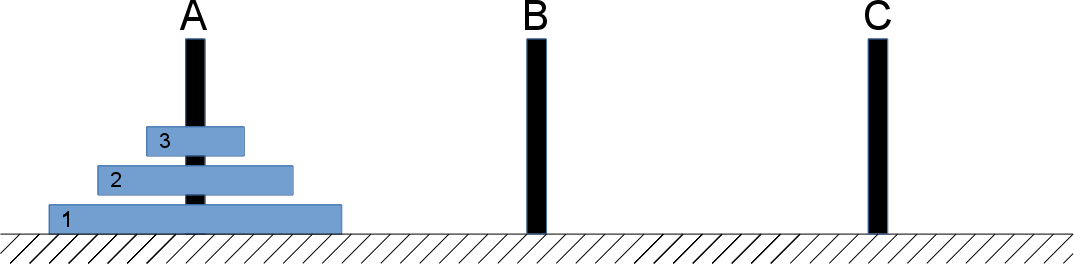
\includegraphics[height=0.3\paperheight]{pucrs-ep-fprog-unidade_01-introducao-laminas-torre_de_hanoi.png}
\end{figure}
\end{frame}

%-------------------------------------------------------
\begin{frame}\frametitle{Torre de Hanói: Solução 1}
\begin{itemize}
	\item Mova o disco menor para o pino mais à direita
	\item Mova o disco médio para o pino central
	\item Mova o disco menor para o pino central (sobre o disco médio)
	\item Mova o disco maior para o pino mais à direita
	\item Mova o disco menor para o pino mais à esquerda
	\item Mova o disco médio para o pino mais à direita
	\item Mova o disco menor para o pino mais à direita
\end{itemize}
\end{frame}

%-------------------------------------------------------
\begin{frame}\frametitle{Torre de Hanói: Solução 2}
\begin{itemize}
	\item Considere:
	\begin{itemize}
		\item os pinos A, B e C
		\item os discos 1, 2 e 3
		\item a operação mover(disco, pino)
	\end{itemize}
	\item A solução consiste nos seguintes passos:
	\begin{itemize}
		\item mover(3, C)
		\item mover(2, B)
		\item mover(3, B)
		\item mover(1, C)
		\item mover(3, A)
		\item mover(2, C)
		\item mover(3, C)
	\end{itemize}
\end{itemize}
\end{frame}

%-------------------------------------------------------
\begin{frame}\frametitle{Desafio 2: Problema do Lobo, da Cabra e do Repolho}
\scriptsize{
\begin{itemize}
	\item Um homem que mora em um lado do rio deseja levar um lobo, uma cabra e um repolho para o outro lado do rio para vendê-los no vilarejo.
	\item Mas a sua canoa não é muito grande e ele terá que atravessar o rio levando apenas um item de cada vez.
	\item E ele não pode deixar a cabra sozinha com o repolho, pois a cabra comeria o repolho.
	\item Da mesma forma ele não pode deixar o lobo sozinho com a cabra, pois o lobo mataria a cabra.
	\item Ajude este homem a resolver este problema: escreva um algoritmo para resolvê-lo!
\end{itemize}
}
\begin{figure}[h]
	\centering
	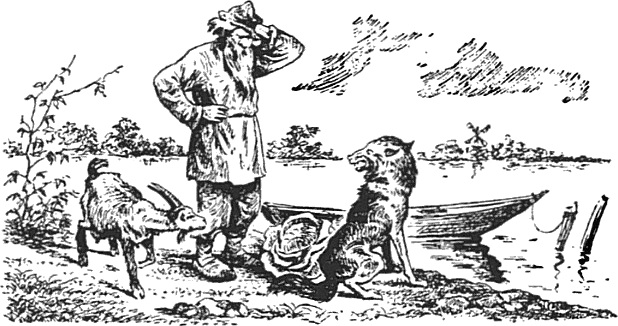
\includegraphics[height=0.3\paperheight]{pucrs-ep-fprog-unidade_01-introducao-laminas-lobo_cabra_repolho.png}\\
	\tiny{\url{https://scientificgems.files.wordpress.com/2014/01/wgc.png}}
\end{figure}
\end{frame}

%-------------------------------------------------------
\begin{frame}\frametitle{Para ajudar na solução de alguns problemas...}
	\begin{block}{Sherlock Holmes --- personagem de Arthur Conan Doyle}
		``Uma vez eliminado o impossível, o que restar, não importa o quão improvável, deve ser a verdade.''
	\end{block}
\end{frame}

%-------------------------------------------------------
\begin{frame}\frametitle{Processo de Desenvolvimento de \emph{Software} {\tiny (HORSTMANN, 2013, p. 19)}}
\begin{figure}[h]
	\centering
	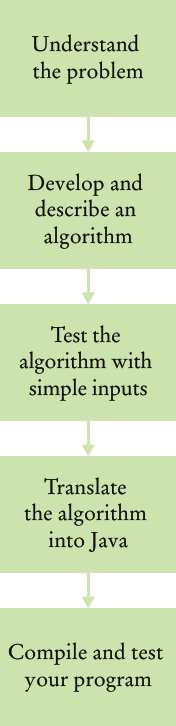
\includegraphics[height=0.7\paperheight]{pucrs-ep-fprog-unidade_01-introducao-laminas-desenvolvimento.png}
\end{figure}
\end{frame}

%-------------------------------------------------------
\begin{frame}\frametitle{Solução de problemas: projeto de algoritmos}
\textbf{Problema:} Você colocou \$10.000 numa conta bancária que recebe 5\% de juros por ano. Quantos anos levará para que você tenha o dobro do valor original?\\
~\\
Como você pode solucionar isto?
\begin{itemize}
	\item método manual: faça uma tabela como a tabela a seguir e acrescente linhas até alcançar o dobro do valor inicial
	\begin{figure}[h]
		\centering
		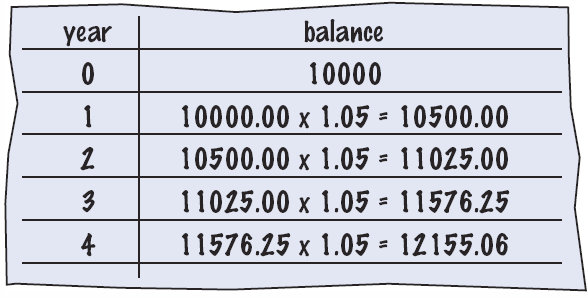
\includegraphics[height=0.25\paperheight]{pucrs-ep-fprog-unidade_01-introducao-laminas-investimento.jpg}
	\end{figure}
	\item use uma planilha: crie uma fórmula para cada linha e repita a fórmula para as demais linhas
\end{itemize}
\end{frame}

%-------------------------------------------------------
\begin{frame}[fragile]\frametitle{Solução de problemas: projeto de algoritmos}
\begin{itemize}
	\item um programa de computador pode automatizar esta tarefa
	\item mas antes precisamos de uma descrição clara e inequívoca, que não necessite de nenhuma adivinhação para ser implementada
	\item o primeiro passo neste sentido é descrever a solução usando \textbf{pseudocódigo}
\begin{verbatim}
Inicie com um valor de ano igual a zero e um total de $10.000
Repita o seguinte enquanto o total seja menor do que $20.000
     Adicione 1 ao valor do ano
     Multiplique o total por 1,05 (crescimento de 5%)
Informe o último valor atribuído ao ano como resposta
\end{verbatim}
\end{itemize}
\end{frame}

%-------------------------------------------------------
\begin{frame}\frametitle{Pseudocódigo}
\begin{itemize}
	\item consiste numa descrição informal de uma sequência de passos para resolver um problema
	\item trata-se de uma descrição que não pode ser entendida diretamente pelo computador, mas que pode ser facilmente convertida para alguma linguagem de programação
	\item é metade do caminho entre a linguagem natural e uma linguagem de programação
	\item deve descrever uma sequência de passos que é inequívoca (não ambígua), executável e finita
\end{itemize}
\end{frame}

%-------------------------------------------------------
\begin{frame}\frametitle{Pseudocódigo}
{\footnotesize Alguns exemplos de construções que aparecem em pseudocódigo são:
\begin{itemize}
	\item obtenção de dados\\
\texttt{Leia as notas do aluno}
	\item definições, atribuições e operações\\
\texttt{custo total = preço de compra + custo operacional\\
Multiplique o subtotal por 1,05\\
Remova o primeiro e o último caracter da palavra}
	\item decisões e repetições\\
\texttt{Se custo total 1 < custo total 2\\
Enquanto o total for menor do que \$10.000\\
Para cada imagem da sequência}
	\item apresentação de resultados\\
\texttt{Escolha o carro 1\\
Informe o último valor atribuído ao ano como resposta}
\end{itemize}}
\end{frame}

%-------------------------------------------------------
\begin{frame}\frametitle{Pseudocódigo}
\begin{itemize}
	\item usa-se indentação (tabulações ou deslocamentos horizontais para a direita) para indicar que comandos ou expressões devem ser selecionados ou repetidos\\
\texttt{Para cada carro\\
~ ~ custo de operação = 10 x custo anual de combustível\\
~ ~ custo total = preço de compra + custo operacional}
	\item aqui a indentação indica que ambas as expressões devem ser executadas para cada carro
\end{itemize}
\end{frame}

%-------------------------------------------------------
\begin{frame}\frametitle{Um problema}
Ler a média de 50 alunos, calculando a média da turma e contando o número de alunos aprovados (com média maior ou igual a 7,0).
\end{frame}

%-------------------------------------------------------
\begin{frame}[fragile]\frametitle{Solução 1: Algoritmo em Português Estruturado}

{\tiny\begin{verbatim}
algoritmo media_de_50_alunos_com_aprovados;
início
    real:    M,    // média de um aluno
             TOT,  // acumulador
             MT;   // média da turma
    inteiro: V,    // variável de controle
             NA;   // número de aprovados

    NA = 0;
    TOT = 0;
    V = 1;
    enquanto (V <= 50) faça
    início
        leia(M);
        se (M >= 7.0) então NA = NA + 1
        TOT = TOT + M;
        V = V + 1;
    fim;
    MT = TOT / 50;
    escreva ("Média da turma = ",MT);
    escreva ("Número de aprovados = ",NA);
fim.
\end{verbatim}}
\end{frame}

%-------------------------------------------------------
\begin{frame}\frametitle{Solução 2: Fluxograma}
\begin{figure}[h]
	\centering
	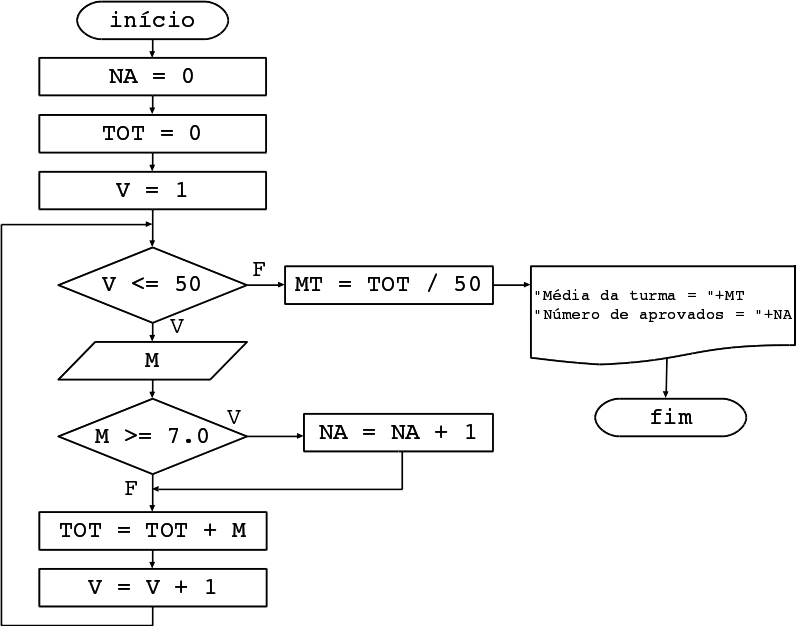
\includegraphics[height=0.65\paperheight]{pucrs-ep-fprog-unidade_01-introducao-laminas-fluxograma.png}
\end{figure}
\end{frame}

%-------------------------------------------------------
\begin{frame}\frametitle{Solução 3: Diagrama de Chapin}
\begin{figure}[h]
	\centering
	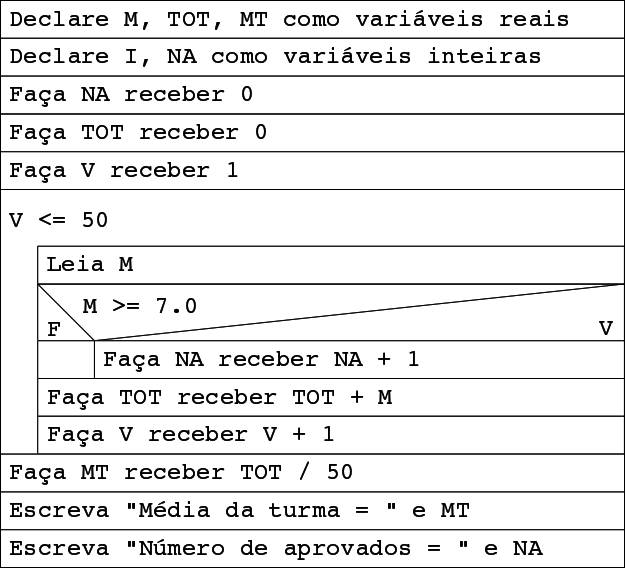
\includegraphics[height=0.65\paperheight]{pucrs-ep-fprog-unidade_01-introducao-laminas-chapin.jpg}
\end{figure}
\end{frame}

%-------------------------------------------------------
\begin{frame}\frametitle{Exercícios}
\begin{enumerate}
	\item Mostre como seria a ``implementação de'' uma solução para resolução de equações do segundo grau, usando a fórmula de Bhaskara, no formato:
	\begin{itemize}
		\item Fluxograma
		\item Diagrama de Chapin
		\item Algoritmo em Português Estruturado
	\end{itemize}
	\item Escreva um algoritmo para calcular e mostrar a soma dos dez primeiros números inteiros positivos: $1 + 2 + 3 + \ldots + 10$.
	\item Escreva um algoritmo para calcular e mostrar o produto dos dez primeiros números inteiros positivos: $1 \times 2 \times 3 \times \ldots \times 10$.
\end{enumerate}
\end{frame}

%-------------------------------------------------------
\begin{frame}[fragile]\frametitle{Resposta do Exercício 1}

{\tiny\begin{verbatim}
algoritmo Bhaskara;
início
    real:    a,b,c,delta,x1,x2;

    leia(a,b,c);
    se (a==0) entao escreva ("Não é uma equacao do segundo grau!");
              senão início
                       delta = b*b - 4*a*c;
                       se (delta<0) então escreva ("Não tem raízes reais!");
                                    senão início
                                             se (delta==0) então início
                                                                    x1 = -b/(2*a);
                                                                    escreva (x1);
                                                                 fim;
                                                           senão início
                                                                    delta = sqrt(delta); // sqrt() = raiz quadrada
                                                                    x1 = (-b+delta)/(2*a);
                                                                    x2 = (-b-delta)/(2*a);
                                                                    escreva (x1,x2);
                                                                 fim;
                                          fim;
                    fim;
fim.
\end{verbatim}}
\end{frame}

%-------------------------------------------------------
\begin{frame}[fragile]\frametitle{Resposta do Exercício 2}

\begin{verbatim}
algoritmo Somatorio_dos_10_primeiros_inteiros_positivos;
início
    inteiro:    i,soma;

    soma = 0;
    i = 1;
    enquanto (i<=10) faça
    início
       soma = soma + i;
       i = i + 1;
    fim
    escreva (soma);
fim.
\end{verbatim}
\end{frame}

%-------------------------------------------------------
\begin{frame}[fragile]\frametitle{Resposta do Exercício 3}

\begin{verbatim}
algoritmo Produtorio_dos_10_primeiros_inteiros_positivos;
início
    inteiro:    i,prod;

    prod = 1;
    i = 1;
    enquanto (i<=10) faça
    início
       prod = prod * i;
       i = i + 1;
    fim
    escreva (prod);
fim.
\end{verbatim}
\end{frame}

%=======================================================
\section{Referências}

%-------------------------------------------------------
\begin{frame}\frametitle{Referências}

\noindent{HORSTMANN, C. \textbf{Java for Everyone – Late Objects}. 2. ed. Hoboken: Wiley, 2013. xxxiv, 589 p.}\\
~\\
\noindent{ORTH, Afonso Inácio. \textbf{Algoritmos e Programação com Resumo das Linguagens PASCAL e C}. Porto Alegre: AIO, 2001. 176 p.}\\
~\\
\noindent{PINTO, Wilson Silva. \textbf{Introdução ao Desenvolvimento de Algoritmos e Estruturas de Dados}. São Paulo: Editora Érica. 1990. 204 p.}

\end{frame}

%=======================================================
\end{document}

